\documentclass[12pt,a4paper]{article}
\usepackage[a4paper]{geometry}
\usepackage{fullpage}
\usepackage{url}
\usepackage[backend=bibtex]{biblatex}
\usepackage{caption}
\usepackage[utf8]{inputenc}
\usepackage{enumerate}
\usepackage{tabularx}
\usepackage{graphicx}
\usepackage{float}
\usepackage{color}
\usepackage{amssymb,amsmath,wasysym}
\usepackage{enumitem}

\addbibresource{bib1.bib}

\begin{document}

\title{Computational Intelligence, SS2017, Assigment 6}

\author{%
\name{Lucas Reeh}
\email{lreeh@student.tugraz.at}
}
\date{\today}

\begin{titlepage}
   \begin{center}
     \begin{huge}
		   %% Update assignment number here
           \textbf{Assignment 6}
     \end{huge}
   \end{center}

   \begin{center}
     \begin{large}
           Computational Intelligence, SS2017
     \end{large}
   \end{center}

   \begin{center}
 \begin{tabularx}{\textwidth}{|>{\hsize=.33\hsize}X|>{\hsize=.33\hsize}X|>{\hsize=.33\hsize}X|} 

           \hline
           \multicolumn{3}{|c|}{\textbf{Team Members}} \\
           \hline
           Last name & First name & Matriculation Number \\
           \hline
           Reeh & Lucas & 00630182 \\
           \hline

     \end{tabularx}
   \end{center}
\end{titlepage}

\tableofcontents
\listoffigures

\newpage

\section{Viterbi Algorithm and optimal State Sequence}
% 
% \begin{figure}[H]
%   \centering
%   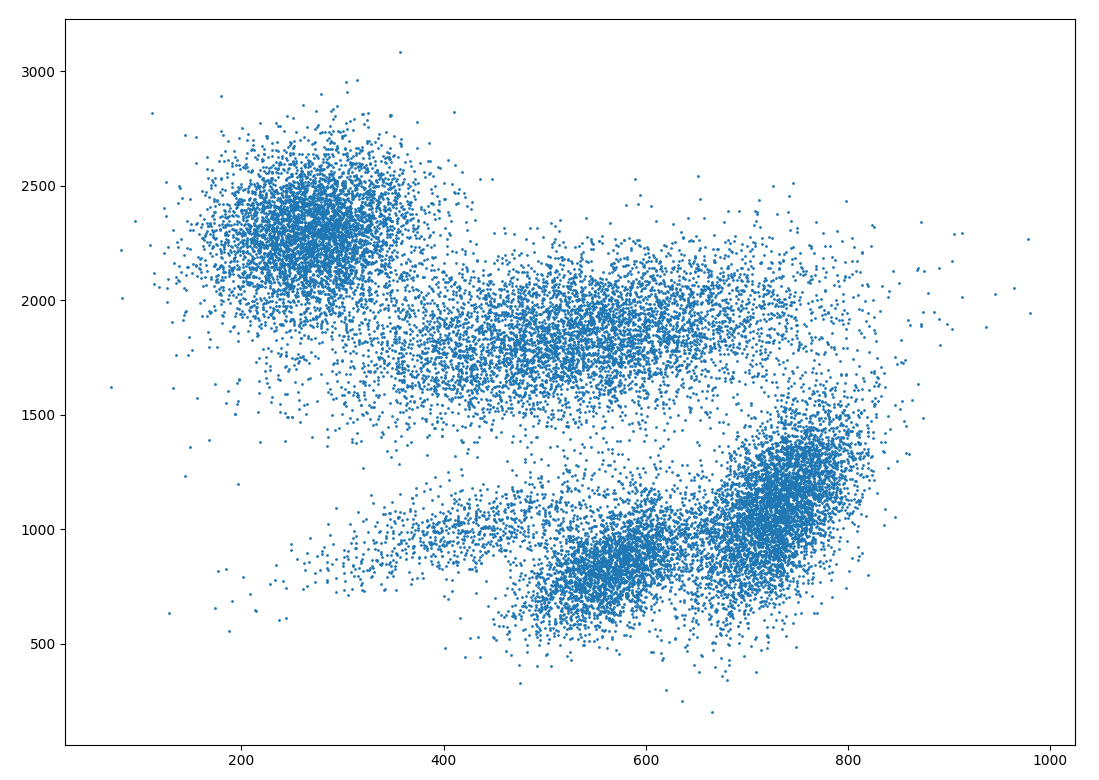
\includegraphics[width=0.8\textwidth]{figures/1_0.png}
% 	\caption{Training Data}
% 	\label{1_0}
% \end{figure}

\setcounter{enumi}{2}
\begin{enumerate}[start=2,label*={\arabic*.}]
  % 1
  % 2
  \item Optimal state sequences\footnote{0 = umbrella, 1 = no
  umbrella}\footnote{r = rainy, s = summy, f = foggy}
  
  \textbf{Result for $\textnormal{HMM}_1$}
  \begin{verbatim}
  X1 = [0, 0, 1, 1, 1, 0]
  q1 = ['r', 'r', 's', 's', 's', 's']
  X2 = [0, 0, 1, 1, 1, 0, 0]
  q2 = ['r', 'r', 'f', 'f', 'f', 'r', 'r']
  \end{verbatim}
  
  \textbf{Result for $\textnormal{HMM}_2$}
  \begin{verbatim}
  X1 = [0, 0, 1, 1, 1, 0]
  q1 = ['r', 'r', 'f', 'f', 'f', 'r']
  X2 = [0, 0, 1, 1, 1, 0, 0]
  q2 = ['r', 'r', 'f', 'f', 'f', 'r', 'r']
  \end{verbatim}
  
  \textbf{Findings}
  
  When observing $X_1$ in $HMM_2$ higher emission probaility for ``no umbrella''
  on foggy days ($0.95$) and higher transition probaility for switching from rain to fog
  ($0.6$) leads to a different path through the states ($n-1$ to $n$) after
  switching observation from $2^{nd}$ day with umbrella to the $3^{rd}$ wihtout.
  Also the probability to stay in state sunny in $HMM_1$ when observing ``no
  umbrella'' is quite high.
  
  Optimal state sequences for observation $X_2$ seems to be no different for
  both models.
  
  \item Numerical instability
  
  Since probability values in each iteration are getting smaller at a certain
  point numerical errors would appear. But if we are only interested in $argmax$
  and $max$ this problem can be avoided by using $log$ for transition and
  emission probabilities without changing our
  results \autocite[373]{Rabiner:1990:THM:108235.108253} (104, 105a-c). This
  scaling method can be further improve as you can see in ``Numerically Stable Hidden Markov Model
Implementation''\autocite{Mann06numericallystable} to fix even more problems
with $log$.

\end{enumerate}


\newpage
\section{Sequence Classification}

\begin{enumerate}[label*={\arabic*.}]
  \item $P(X|\mathbf{\Theta_i})$
\begin{align*}
P(X|\mathbf{\Theta_i}) & = \sum_{\mathbf{Q}\in\mathcal{Q}}
P(X, \mathbf{Q}|\mathbf{\Theta_i})
\end{align*}
With $\mathit{Q}$ being the set of all state sequences. This would be very
expensive to compute because of the exponential amount of sequences
$|\mathcal{Q}| = (N_s)^N$. With naive marginalisation this would result in
$\mathcal{O}(2N(N_s)^N)$ operations\autocite{lecuter_notes_spsc}.

  \item Joint probability
\begin{align*}
P(X|\mathbf{\Theta_i}) & = \sum_{\mathbf{Q}\in\mathcal{Q}}
P(X, \mathbf{Q}|\mathbf{\Theta_i})\\
& = \sum_{\mathbf{Q}\in\mathcal{Q}}
P(X|\mathbf{Q},\mathbf{\Theta_i})P(\mathbf{Q}|\mathbf{\Theta_i})
\end{align*}

So viterbi-algorithm already holds an approximation for $\mathcal{Q}_N$ after
computing $\delta_N$ (max probability for partial sequences). The last
observation can be used for classification when assuming the probability
along the best path.

 \item Classification

 \textbf{Result for $X_1$}
  \begin{align*}
P(X_1 | \textnormal{HMM}_1) & = 0.0020198\\
P(X_1 | \textnormal{HMM}_2) & = 0.0008406\\
& \implies \textnormal{best is } \textnormal{HMM}_1 
\end{align*}

 \textbf{Result for $X_2$}
  \begin{align*}
P(X_2 | \textnormal{HMM}_1) & = 0.0004099\\
P(X_2 | \textnormal{HMM}_2) & = 0.0004062\\
& \implies \textnormal{best is } \textnormal{HMM}_1 \quad\textnormal{(seems
wrong?)}
\end{align*}

\end{enumerate}

\newpage
\section{Samples from a Gaussian Mixture Model}

\begin{enumerate}[label*={\arabic*.}]
  \item Examples for Sampling\footnote{u = umbrella, nu = no
  umbrella}\footnote{r = rainy, s = summy, f = foggy}
  \begin{verbatim}
Sampling from HMM1
['nu', 'u', 'u', 'nu', 'nu']
['r', 'r', 'r', 's', 's']
Sampling from HMM2
['nu', 'u', 'nu', 'nu', 'u']
['f', 'r', 'f', 'f', 'r']
  \end{verbatim}
  \item Same procedure as used as for GMM sampling: Piped usage of discrete
  sampling (with provided function). First draw for emission probability and
  transition probability and then draw depending on that every N-th sample (in
  GMM it was first distribution and depending on this the second and so on
  \ldots).
\end{enumerate}

\newpage
\section{Markov Model}

\begin{enumerate}[label*={\arabic*.}]
  \item Compute $P_2$ and $P_3$ (Markov-Chain)
    \begin{align*}
P_1 &=
\begin{bmatrix}
\frac{1}{3}\\
\frac{1}{3}\\
\frac{1}{3}
\end{bmatrix}\\
P_2 &= \pi_1 \cdot A\\
P_2 &= 
\begin{bmatrix}
0.4\\
0.31\dot6\\
0.28\dot3
\end{bmatrix}\\
P_3 &= \pi_1 \cdot A^2\\
P_3 &= 
\begin{bmatrix}
0.24\\
0.1508\dot3\\
0.10416\dot6
\end{bmatrix}\\
\end{align*}
  \item $P_n$ only works for countable infitie state transitions (Markov-Chain)
\begin{align*}
P_{n+1} &= \pi_1 \cdot A^{n-1}\\
\end{align*}
or if you shift the index
\begin{align*}
P_0 &= \pi_0\\
P_n &= \pi_0 \cdot A^{n}\\
\end{align*}
\end{enumerate}

\newpage
\printbibliography

\end{document}